\documentclass[14pt]{extreport}
\usepackage{fontspec}
\usepackage{polyglossia}
\setmainlanguage{russian}
\setotherlanguages{english}

\setmainfont{Times New Roman}
\newfontfamily\cyrillicfont{Times New Roman}
\newfontfamily\cyrillicfontsf{Times New Roman}
\newfontfamily\cyrillicfonttt{Times New Roman}

\usepackage{indentfirst}
\setlength{\parindent}{1.25cm}
\setlength{\parskip}{0pt}
\linespread{1.5}
\usepackage[a4paper,left=30mm,right=10mm,top=20mm,bottom=20mm]{geometry}
\usepackage{graphicx}

\begin{document}

МИНИСТЕРСТВО НАУКИ И ВЫСШЕГО ОБРАЗОВАНИЯ \\
РОССИЙСКОЙ ФЕДЕРАЦИИ \\
ФЕДЕРАЛЬНОЕ ГОСУДАРСТВЕННОЕ БЮДЖЕТНОЕ ОБРАЗОВАТЕЛЬНОЕ УЧРЕЖДЕНИЕ ВЫСШЕГО ПРОФЕССИОНАЛЬНОГО ОБРАЗОВАНИЯ \\
«РОССИЙСКИЙ ГОСУДАРСТВЕННЫЙ ПЕДАГОГИЧЕСКИЙ УНИВЕРСИТЕТ им. А. И. ГЕРЦЕНА» \\
Институт информационных технологий и технологического образования \\
Кафедра компьютерные технологии и электронного обучения \\
Основная профессиональная образовательная программа \\
Направление подготовки 09.03.01 Информатика и вычислительная техника \\
Направленность (профиль) «Технологии разработки программного обеспечения» \\
форма обучения - очная \\

\vspace{10mm}

\begin{center}
КУРСОВАЯ РАБОТА \\
по дисциплине: «Технологии компьютерного моделирования» \\
«Распознавание текста» \\
\end{center}

\vspace{20mm}

Автор работы студент 2 курса \\
2 группы \\
\_\_\_\_\_\_\_\_\_\_\_\_ Р.М. Суворов \\
Руководитель: \\
\_\_\_\_\_\_\_\_\_\_\_\_ Е.З. Власова \\
«\_\_\_» \_\_\_\_\_\_\_\_\_ 2024 г \\

\vspace{20mm}

\begin{center}
Санкт-Петербург \\
2024
\end{center}

\newpage

\tableofcontents

\newpage

\chapter*{Введение}
\addcontentsline{toc}{chapter}{Введение}

В современном мире распознавание текста играет ключевую роль во многих областях, включая сканирование документов, системы безопасности, исследования в области искусственного интеллекта и многое другое. Целью данного исследования является изучение и реализация метода распознавания текста с использованием технологий компьютерного моделирования. Это поможет понять основные принципы работы систем распознавания текста и применить полученные знания на практике для создания эффективных решений.

Задачи:
\begin{itemize}
    \item Проанализировать литературу по теме, чтобы составить обзор существующих методов и подходов к распознаванию текста.
    \item Рассмотреть математическую модель.
    \item С использованием языка программирования Python реализовать алгоритмы распознавания текста на основе полученных знаний. Это позволит провести вычисления и анализ результатов.
    \item Сделать выводы о применимости и эффективности разработанных методов распознавания текста и определить возможные направления для дальнейших исследований.
\end{itemize}

\chapter{Распознавание текста}
Распознавание текста - это процесс автоматического определения содержания или категории текстовых данных с помощью компьютерных алгоритмов. Он может включать в себя различные методы анализа, такие как обработка естественного языка, машинное обучение и статистические модели. Распознавание текста широко применяется в таких областях, как поисковые системы, автоматическая обработка документов и многое другое. 

В данной работе мы будем использовать метод евклидова расстояния. Распознавание текста по фото - это метод классификации или распознавания, основанный на анализе изображений, содержащих текстовую информацию. В этом методе изображение с текстом представляется как вектор, в котором каждая компонента соответствует некоторому признаку или характеристике изображения, например, интенсивности пикселей или форме символов.

Идея заключается в следующем: каждое изображение с текстом анализируется с помощью алгоритмов компьютерного зрения для извлечения текстовой информации. Затем этот текст преобразуется в числовой вектор, который может быть использован для классификации или распознавания.

Хотя метод распознавания текста по фото требует дополнительной обработки изображений и может сталкиваться с проблемами, такими как шум или неправильное распознавание символов, он широко используется в таких областях, как оптическое распознавание символов (OCR), считывание номеров автомобилей, а также в приложениях для мобильных устройств.


\chapter{Реализация решения}

\section{Реализация логики}
\subsection{Подготовка данных (build.py):}
Изображения из папки letters разбиваются на квадраты размером 32x32 пикселя. Каждый квадрат преобразуется в массив пикселей в оттенках серого. Для каждого пикселя вычисляется среднее значение. Полученные средние значения записываются в файл res.csv, который содержит информацию о средних значениях пикселей для каждого символа.

\subsection{Распознавание текста (main.py):}
Входное изображение разбивается на отдельные символы. Для каждого символа извлекается массив пикселей. Вычисляется евклидово расстояние между массивом пикселей символа и эталонными массивами из файла res.csv по формуле:

\[
d = \sqrt{\sum_{i=1}^{n}(x_i - y_i)^2}
\]

По минимальному расстоянию определяется наиболее похожий символ для каждого изображенного символа. Формируется распознанный текст на основе найденных символов.

\section{Реализация программы}
Для реализации проекта была разработана программа на языке Python с использованием следующих библиотек:
\begin{itemize}
    \item Pillow — для обработки изображений,
    \item csv — для работы с файлами формата CSV,
    \item os — для взаимодействия с операционной системой.
\end{itemize}

Ссылка на Github репозиторий с кодом программы: \url{https://github.com/webbsalad/text_recognition/tree/main}


В нашем случае тестовый пример состоит из 113 символов, программа допускает 2 ошибки, что означает, что точность программы равна:

\[
\frac{113 - 2}{113} \times 100 = 98\%
\]

Ответ программы верный на 98\%. Это показывает высокую точность разработанного алгоритма распознавания текста и подтверждает эффективность использованных методов. В дальнейшем возможно совершенствование алгоритмов для повышения точности и расширение их применения на более сложные задачи распознавания текста.

\begin{figure}[h]
\centering
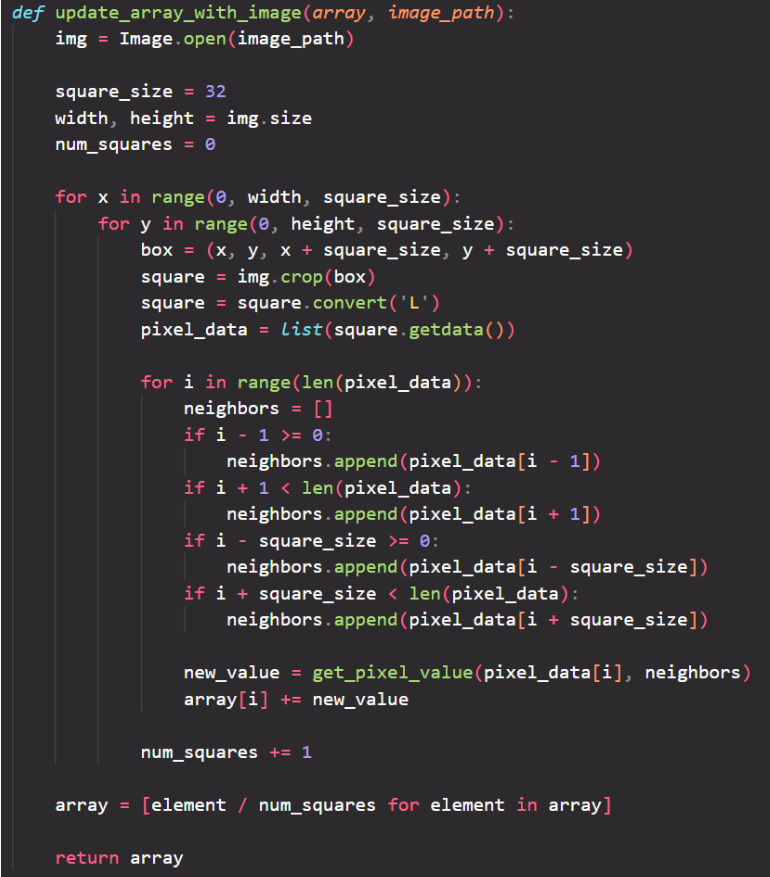
\includegraphics[width=0.5\textwidth]{photos/image1.png}
\caption{Пример кода}
\label{fig:example}
\end{figure}


\begin{table}[h]
\centering
\begin{tabular}{|c|c|c|}
\hline
№ & проценты & колличество \\
\hline
1 & 98 & 1 \\
\hline
\end{tabular}
\caption{Пример таблицы}
\label{tab:example}
\end{table}

\chapter*{Заключение}
\addcontentsline{toc}{chapter}{Заключение}

В ходе выполнения курсовой работы были изучены и решены следующие задачи:
\begin{itemize}
    \item Изучена тема распознавания текста, включая основные методы и подходы.
    \item Рассмотрена математическая модель распознавания текста.
    \item С использованием языка программирования Python реализованы алгоритмы распознавания текста, проведены вычисления и анализ результатов.
    \item Сделаны выводы о эффективности разработанных методов распознавания текста и определены возможные направления для дальнейших исследований благодаря полученному результату, приближенному к оптимальным показателям.
\end{itemize}

\chapter*{Список литературы}
\addcontentsline{toc}{chapter}{Список литературы}
\begin{enumerate}
    \item Pillow: сайт. - 2022. - URL: \url{https://pillow.readthedocs.io/en/stable/} (дата обращения: 20.05.2024)
    \item Wikipedia.org: сайт. - 2012. - URL: \url{https://ru.wikipedia.org/wiki/Евклидова_метрика} (дата обращения: 20.05.2024)
    \item Python Documentation: сайт. - 2023. - URL: \url{https://docs.python.org/3/library/csv.html} (дата обращения: 20.05.2024)
    \item Habr: сайт. - 2024. - URL: \url{https://habr.com/ru/articles/} (дата обращения: 20.05.2024)
    \item Python.org: сайт. - 2024. - URL: \url{https://www.python.org/} (дата обращения: 20.05.2024)
    \item Visual Studio Code Documentation: сайт. - 2024. - URL: \url{https://code.visualstudio.com/docs} (дата обращения: 20.05.2024)
    \item Microsoft Learn: сайт. - 2024. - URL: \url{https://learn.microsoft.com/} (дата обращения: 20.05.2024)
    \item GitHub: сайт. - год не указан. - URL: \url{https://github.com/} (дата обращения: 20.05.2024)
    \item Английский алфавит в Википедии: сайт. - 2012. - URL: \url{https://ru.wikipedia.org/wiki/английский_алфавит/} (дата обращения: 20.05.2024)
    \item GitHub: сайт. - год не указан. - URL: \url{https://pillow.readthedocs.io/en/stable/reference/Image.html} (дата обращения: 20.05.2024)
\end{enumerate}

\end{document}
